\documentclass[tikz,margin=0pt,dvipsnames,rgb]{standalone}

\usepackage{amsmath,amssymb,amsfonts}
\usetikzlibrary{calc,
fit,
shapes.misc,
shapes.geometric,
arrows.meta,
fadings,
matrix,
chains,
scopes,
positioning}

\usepackage{pgfplots}
\usepackage{pgfplotstable}
\pgfplotsset{compat=1.18}



\usepackage[]{fontspec}

\setmainfont{Latin Modern Roman}
\setmonofont{Latin Modern Math}
\renewcommand{\textsc}[1]{{\fontfamily{lmr}\selectfont \scshape #1}}

\usepackage[]{bm}

\makeatletter
\@ifundefined{fromRoot}{\newcommand{\fromRoot}[1]{../../#1}}{}

\def\input@path{{../..}{..}{.}{./svg}{./pgfplots}{./tikzpicture}}
%or: \def\input@path{{/path/to/folder/}{/path/to/other/folder/}}
\makeatother

\newcommand*{\gf}[1]{\acrshort{gf}($#1$)}%
\newcommand*{\mpn}[1]{\bm{P}_{#1}}%
\newcommand*{\pn}[1]{%
  \ifthenelse{\equal{#1}{}}{$\mpn{0}$}{$\mpn{#1}$}%
}%

\newcommand*{\pk}[3]{%
  \ifthenelse{\equal{#1}{#2}}{\textcolor{red}{\phantom{.}$p_0$\phantom{.}}}{\phantom{.}$p_#3$\phantom{.}}%
}%


\newcommand*{\placeholder}{
\includegraphics[width=\linewidth, height=.25\textheight, keepaspectratio = true]{figures/certified_xilinx.png}}%

\newcommand*{\snr}{\acrshort{snr}}%
\newcommand*{\snrs}{\acrshortpl{snr}}%

\newcommand*{\mpd}[0]{p_\Delta}%
\newcommand*{\mpo}[0]{p_\omega}%
\newcommand*{\pd}[0]{$\mpd$}%
\newcommand*{\po}[0]{$\mpo$}%
\newcommand*{\mpfa}[0]{\mathcal{P}_{fa}}%
\newcommand*{\mpmd}[0]{\mathcal{P}_{md}}%
\newcommand*{\pfa}[0]{\acrshort{pfa}}%
\newcommand*{\pmd}[0]{\acrshort{pmd}}%
\newcommand*{\mnorm}[1]{\mathcal{L}_{#1}}%
\newcommand*{\norm}[1]{$\mnorm{#1}$}%
\newcommand*{\fft}{\acrshort{fft}}%
\newcommand*{\mfft}[1]{\mathcal{F}(#1)}%
\newcommand*{\mifft}[1]{\mathcal{F}^{-1}(#1)}%
\newcommand*{\ts}{\acrshort{ts}}%

\newcommand*{\cpp}[1]{C\textrm{++#1}}%
\newcommand*{\na}{\textrm{\textcolor{SlateGray4}{N/A}}}%

\newcommand*{\vect}[1]{\bm{#1}}%
\newcommand*{\mat}[1]{\bm{\mathrm{#1}}}%

\newcommand*{\task}[1]{\mathcal{T}_{#1}}%

\newcommand*{\sdr}{\acrshort{sdr}}%
\newcommand*{\fpga}{\acrshort{fpga}}%



\begin{document}
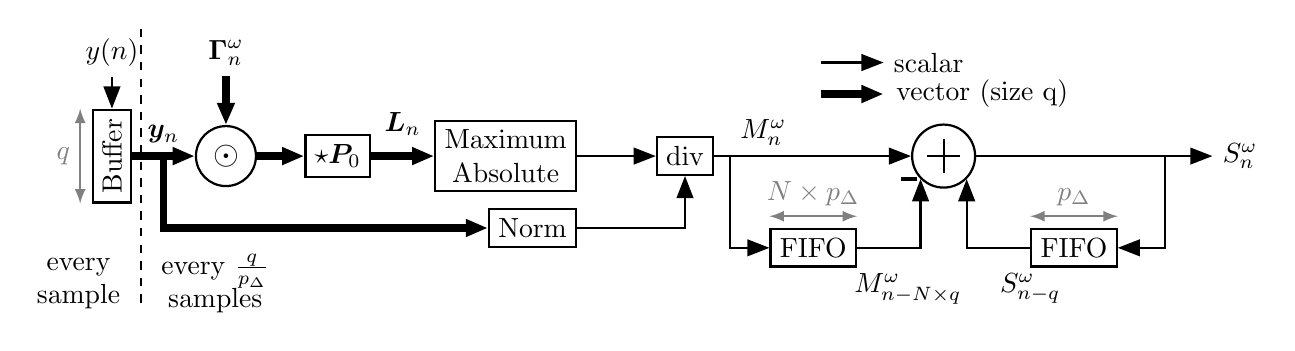
\begin{tikzpicture} [->,
  >={Triangle[width = 6pt, length = 8pt]},
  auto,
  thick,
  main node/.style={rectangle, fill = white!35, draw,
      align=center}]

  \node [pos=0, left] (yn) at (0,0) {$y(n)$};

  \node [main node,
    rotate = 90,
    anchor = east
    % below = .8 cm of yn
  ] (pack) at ($(yn.south) + (0, -.4)$) {Buffer};

  \node [circle, draw,
    % fill = gray!40!white, 
    align = center,
    minimum size = .7 cm,
    right = .8 cm of pack.south
  ] (multf) {\large $\odot$};
  %\draw [-] ($(multf.north east) + (-.1, -.1)$) -- ($(multf.south west) + ( .1, .1)$);
  %\draw [-] ($(multf.north west) + ( .1, -.1)$) -- ($(multf.south east) + (-.1,  .1)$);

  \node [] (gamma) at (multf |- yn) {$\vect{\Gamma}^\omega_n$};
  \draw [line width = 2.6pt] (gamma.south) -> (multf.north);

  \node [main node,
    % fill = gray!40!white, 
    align = center,
    right = .6 cm of multf
  ] (corr) {$\star \vect{P}_0$};


  \draw [dashed, -] ($(yn.north east) + (-0.1, 0)$) -> ($(yn.north east) + (-.1, -3.5)$)
  node [pos=1, anchor = south] (ankdsh) {};
  \node [draw = none, anchor = east, align = center] at (ankdsh.north west) {every\\ sample};
  \node [draw = none, anchor = west, align = center] at (ankdsh.north east) {every $\frac{q}{p_\Delta}$\\samples};


  \draw (yn.south) -> (pack.east);
  \draw [line width = 2.6pt] (multf.east) -> (corr.west);

  \draw [line width = 2.6pt] (pack.south) -- (multf.west)
  node [midway, anchor = south, align=center] (vyn) {$\vect{y}_n$};

  \node [main node,
    align = center,
    % fill = gray!40!white, 
    right = .8cm of corr
  ] (mabs) {Maximum\\Absolute};

  \draw [line width = 2.6pt] (corr.east) -- (mabs.west)
  node [midway, above = .1 cm, align=center] () {$\vect{L}_n$};

  \node [main node,
    % fill = gray!40!white, 
    anchor = north east
  ] (norm) at ($(mabs.south east) + (0, -.2)$) {Norm};

  \draw [line width = 2.6pt] (vyn.south) |- (norm.west);

  \node [main node,
    draw,
    % fill = gray!40!white, 
    %minimum width = 2cm,
    right = 1cm of mabs
  ] (div) {div};

  \draw (norm.east) -| (div.south)
  node [pos=0, right = .15, align=center] () {};
  \draw (mabs.east) -- (div.west)
  node [pos=.6, above = .2cm, align=center] () {};


  \node [circle,
    draw,
    % fill = gray!40!white, 
    minimum size = .8cm,
    right = 2.5 cm of div
  ] (add)   {};
  \draw [-] ($(add.north) + ( 0, -.2)$) -- ($(add.south) + (  0, .2)$);
  \draw [-] ($(add.west)  + (.2,   0)$) -- ($(add.east)  + (-.2,  0)$);


  \node [main node,
    % fill = gray!40!white, 
    anchor = north east
  ] (ff) at ($(add.south) + (-1.1, -.5)$) {FIFO};

  %   \node [] () at ($(add.south west) + ( - .2, 0)$) {\Huge $\vect{-}$};
  \draw [-, ultra thick] ($(add.south west) + ( - .25, 0)$) --  ($(add.south west) + ( - .05, 0)$);
  % \node [] () at ($(add.south west) + (-.4,   0)$) {$+$};
  % \node [] () at ($(add.north west) + (  0,  .4)$) {$+$};

  \draw (div.east) -- (add.west)
  node [pos = .25, above] () {$M^\omega_{n}$};

  \draw ($(div.east) + (.2, 0)$) |- (ff.west);
  \draw (ff.east) -| (add.south west)
  node [pos=0.4, below = .2] () {$M^\omega_{n - N \times q}$};


  % \node [main node,
  %   % fill = gray!40!white, 
  %   minimum size = .75cm,
  %   minimum height = 1.5cm
  % ] (reg) at ($(add.north east) + (.5, 1.75)$) {R};

  \node [right = .5 cm of add] (ankh4) {};

  \node [main node,
    anchor = north west,
  ] (regq) at ($(add.south) + (1.1, -.5)$) {FIFO};
  %\node [isosceles triangle,
  %  rotate=180,
  %  isosceles triangle apex angle=60,
  %  draw,
  %  anchor=west
  %] () at ($({reg}.east) + (0, -.5)$) {};

  \node [right = 3cm of add] (out) {$S^\omega_n$};
  \draw (add.east) -- (out.west);

  \draw ($(add.east -| regq.east) + (.6, 0)$) |- (regq.east);
  \draw (regq.west) -| (add.south east)
  node [pos=0, below = .2] () {$S^\omega_{n - q}$};

  \draw ($(mabs.south) + (4, 1.65)$) -> ($(mabs.south) + (4.8, 1.65)$)
  node [pos = 1, right] (scalar) {scalar};

  \draw [line width = 2.6pt] ($(mabs.south) + (4, 1.25)$) -> ($(mabs.south) + (4.8, 1.25)$)
  node [pos = 1, right] (lq) {vector (size q)};

  \draw [latex-latex, gray] ($(ff.north west) + (0, +.15)$) -- ($(ff.north east) + (0, +.15)$)
  node [midway, above] {$N \times p_\Delta$};
  \draw [latex-latex, gray] ($(regq.north west) + (0, +.15)$) -- ($(regq.north east) + (0, +.15)$)
  node [midway, above] {$p_\Delta$};

  \draw[gray, latex-latex] ($(pack.north west) + (-.15, 0)$) -- ($(pack.north east) + (-.15, 0)$)
  node [midway, left] () {$q$};

\end{tikzpicture}

\end{document}